\section{Methodology}
\label{sec:methodology}

As already alluded to in \autoref{sec:introduction} the goal of the project is to
analyse commit messages. To achieve this repositories of the top 10 most
wanted languages. The reason for using this list as reference, is because it
has a great assortment of languages that are in high demand and also relevant
in today's development climate. The languages in question are:

\begin{figure}[H]
  \centering
  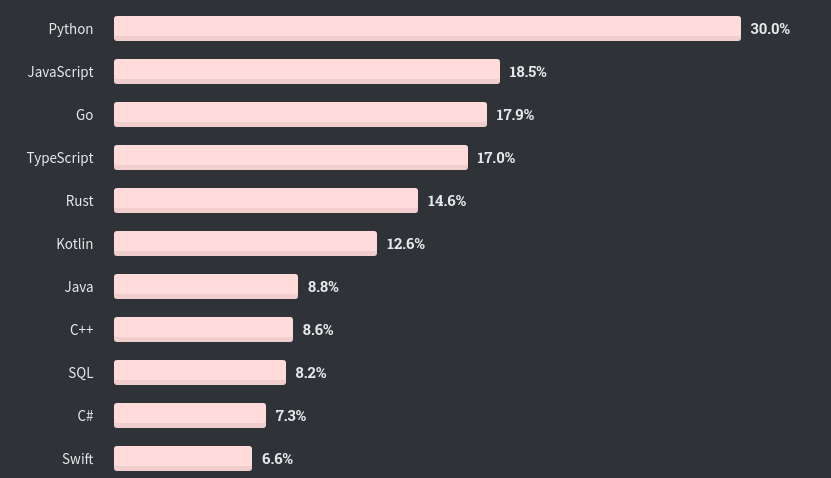
\includegraphics[width=\textwidth]{wanted_languages.png}
  \caption{top 10 most wanted languages \cite{so-survey}}
  \label{fig:wanted_languages}
\end{figure}

It has to be noted that not all laguages depicted in
\autoref{fig:wanted_languages} have been chosen since SQL is not suited for
analysis and therefore Swift has been chosen instead. Regardless of the
percentages seen in \autoref{fig:wanted_languages}, 100000 commits of each
language have been considered for analysis, where 10000 is the maximum per
repository. To further diversify the results a limit has been imposed regarding
the amount of commits per author.

The language of choice for the programming part of the analysis
is Python. Python is well suited for this project as it has rich support for
natural language processing related tasks. Additionally the language is great
for quick prototyping of ideas and with the help of tools like Jupyter
Notebook, document with graphs and text can be created in no time. Especially
during the scraping process the library PyGithub was put to good use. PyGithub
is a Python library that offers typed interactions with the GitHub API v3
\cite{pygithub}. The results of the fetching process are furthermore cached in
one CSV file per language.

